\chapterpicture{header_11}
\chapter{Farmaci antitumorali}
\markboth{Farmaci antitumorali}{\printitle}

Il cancro è una delle principali cause di morte nel mondo. Alcuni
sinonimi sono neoplasia (quando si forma qualcosa di nuovo), quindi si
ha una proliferazione di cellule tumorali, cancro o tumore.

In base alla tipologia di cellule si avrà un determinato tipo di tumore,
che possono essere benigni o maligni. I tumori maglie hanno una velocità
di proliferazione maggiore rispetto a uno benigno, e che quindi può
causare delle metastasi nel corpo.

Tra le cause note, vi sono:
\begin{itemize}
\item
  Fumo
\item
  Alimentazione. Non solo corretta, ma anche se si introducono troppi
  grassi, o altre sostanze
\item
  L'ambiente. Vivere in una città inquinata aumenta l'incidenza.
  L'inquinamento chimico è anche un'altra causa dei tumori.
\item
  Virus. Non sono da considerare una causa minore, come EBV (herpes),
  HIV, HBV (epatiti), HPV (papilloma) \ldots Ad esempio il virus
  dell'herpes può portare a un tumore alla gola (dopo molti anni).
\end{itemize}

Una cosa da considerare sono gli oncogeni e gli oncosoppressori mutati
(mutazioni genetiche). Alcune proteine regolano la crescita cellulare,
quindi le proteine devono essere espresse nel modo giusto per poter
discriminare la vita della cellula. Se avvengono delle mutazioni, si
può avere una iperproduzione che replicano la cellula, quindi più
replicazione comporta una maggiore incidenza di tumori.

Le proteine
possono quindi cambiare in modo anomalo, portando a proliferazione
accelerata. Dall'altra parte vi sono gli oncosoppressori, che sono
quei geni che codificano proteine che eliminano la cellula quando
subisce delle mutazioni. Il processo è definito \emph{apoptosi}, che
consente alla cellula di morire, se troppo compromessa. Se gli
oncosoppressori subiscono delle mutazioni, è possibile che siano
ridotti e quindi la cellula con le mutazioni replica, portando alla
formazione di un maggior numero di cellule che possono generare
tumori. Sia oncosoppressore, che proto-oncogeni possono riferirsi ai
geni o alle proteine.

I difetti genetici portano ai difetti cellulari. Si possono avere le vie
di trasduzione del segnale alterato, l'ipersensibilità alla crescita, le
alterazioni nella regolazione del ciclo cellulare. Le cellule tumorali
sono immortali, nel senso che sono molto rapide a dividersi.

I tumori sono solitamente accompagnati da angiogenesi, ovvero la
formazione di nuovi vasi sanguigni attorno al tumore. Attraverso il
flusso sanguigno si possono disperdere e generare tumori secondari.

Le cellule tumorali possono avere una varietà molto ampia, però le
cellule tumorali hanno delle caratteristiche in comune. Lista nelle
slides. Le cellule possono riprogrammare l'equilibrio energetico e la
capacità di sfuggire al sistema immunitario.

Questo, se ci sono delle cellule difettose, è responsabile
dell'eliminazione di queste cellule. Se le cellule sono tante e molto
veloci a riprodursi, non riescono a stare dietro.

\section{Riprogrammazione del metabolismo}

Le cellule tumorali hanno un pH più acido rispetto a quelle normali. Le
cellule tumorali producono energia per glicolisi. Il processo richiede
dell'energia iniziale, però poi si ha la produzione di due unità di ATP
in più. La cellula tumorale utilizza molto glucosio per i processi di
proliferazione. Le cellule tumorali determinano un consumo molto elevato
di glucosio\footnote{Motivo per non mangiare molto zucchero}. La
glicolisi è un processo anaerobico, dei ricercatori hanno determinato
che la glicolisi avviene anche in presenza di ossigeno. Questo è noto
come il paradosso di Warburg, che dice che nelle cellule tumorali
avviene la glicolisi aerobica; quindi anche se si può avere un processo
aerobico, ne avviene uno anaerobico.

\begin{figure}[H]
  \centering
  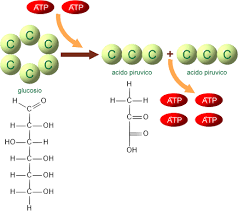
\includegraphics[width=0.5\textwidth]{19_001}
\end{figure}

La glicolisi porta alla produzione di acido lattico, e avvengono altri
processi che portano alla produzione di sostanze acide, questo causa
l'accumulo di acidi che abbassano il pH della cellula.

Questa caratteristica può essere sfruttata, per dei sistemi di drug
delivery, quindi per spostare il farmaco dove il pH è acido, lasciando
intatte le cellule con il pH normale. Questo però dipende dalla
tipologia di tumore e dal grado di conoscenza della patologia; però ora
come ora, non sono molto specifiche.

Le terapie sono: 
\begin{itemize}
\item Chirurgia 
\item Radioterapia
\item Chemioterapia
\end{itemize}

Noi siamo interessati alla chemioterapia. I farmaci in elenco sono
elencati nella lista.

Quindi si hanno i farmaci che agiscono sugli acidi nucleici:

\begin{itemize}
\item \emph{Farmaci antimetaboliti}\ft{Come gli antiestrogeni, che sono farmaci usati per la cura di alcuni tumori, mammella, si può bloccare
la produzione di estrogeni. Solo alcuni tumori utilizzano questo
pathway.}. Vanno ad agire sui metaboliti della cellula, che
quindi sono abbastanza specifici.
Altri farmaci agiscono su altre proteine strutturali
\item \emph{Inibitori delle vie di trasduzione del segnale.} Un esempio è Imatinib, che è un inibitore
delle chinasi.
\item Poi ci sono altri \emph{inibitori enzimatici vari}, si usano se sono note le
alterazioni causate dai tumori
\item \emph{Terapia immunologica.} Utilizzo di anticorpi monoclonali. Alcuni tumori
presentano degli antigeni selettivi, quindi si sono sviluppati degli
anticorpi che legano questi antigeni. Questa terapia può essere
applicata solo ad alcuni tipi di tumori.
\item \emph{Terapia genica.} Si ha un target, che è il genoma della cellula tumorale
stessa, e si cerca di silenziarlo tramite delle molecole, che però sono
acidi nucleici. Queste sequenze sono modificate per resistere ai sistemi
di difesa del corpo. Diventano la parte complementare dell'RNA, che
codifica per determinate proteine, che non vogliamo che vengano
sovraespresse. La sovraespressione può causare il tumore. Le macchine
molecolari per la sintesi proteica non riescono a leggere queste
sequenze di RNA
\end{itemize}


I farmaci che agiscono direttamente negli acidi nucleici sono:
\begin{itemize}
\item \emph{Alchilanti:} interagiscono attraverso dei legami covalenti
\item \emph{Leganti reversibili:} interagiscono con dei legami deboli, quindi con la 
doppia elica 
\item \emph{Tagliatori di catena:} causano dei danni alla catena di DNA con
la produzione di radicali 
\item \emph{ASO, oligonucleotidi antisenso}, che vanno ad
appaiarsi al DNA
\item  \emph{RNAi} RNA interference. Silenziano alcune proteine. Il
processo avviene normalmente, in quanto non tutto il DNA che abbiamo va
a codificare proteine, ma altre regolano l'espressione genica. Quindi
queste parti vanno eliminate
\end{itemize}

\section{Alchilanti}

Il cloro è stata una delle prime armi usate. Un altro gas è il gas
mostarda, o iprite, che deriva da Ypres. È anche un agente alchilante
del DNA.
Non è realmente un gas, ma è un liquido. Ha un odore simile all'aglio
(mostarda).

È un agente urticante, non uccideva subito, ma aveva un azione nel
seguito della battaglia.

È stato pensato l'uso dell'iprite per la leucemia, ma è risultato
tossico.

Nella seconda guerra mondiale, non ci sono stati utilizzi di armi
chimiche, però entrambe le parti avevano l'accesso e il possibile
utilizzo delle armi chimiche, tramite l'uso dell' N-LOST. Gli americani
lo possedevano in una nave, però non hanno mai dichiarato che era
presente. In seguito ad un incidente, si è visto che alcune persone
soffrono dei sintomi delle N-LOST.

Le cellule tumorali sono più soggette ad agenti alchilanti del DNA,
quindi si potrebbero usare come trattamento per i tumori. Gli
elettrofili sono particolarmente reattivi, quindi tossici per il DNA.

Lo scheletro del DNA si vede che la base azotata è soggetta ad attacchi
nucleofili. In particolare, l'azoto 7 è molto più reattivo, perché è
presente il sistema \pi. Un altro punto di attacco per i nucleofili è
l'ossigeno del fosfato, in quanto è carico.

Gli acidi/basi usano la pka per determinare se un acido è forte o
debole.

I nucleofili e gli elettrofili non hanno a che fare con una costante, ma
si guarda la cinetica.

Quindi alcuni elettrofili preferiscono reagire con l'ossigeno o con
l'azoto. L'ossigeno carico preferisce nucleofili hard, mentre l'azoto
del sistema \pi{} preferisce nucleofili soft. QUindi si può lo stesso
metilare il gruppo fosfato.

La metilazione comporta problemi con la riproduzione del DNA, anche se
il cambiamento è piccolo. In particolare questo comporta anche un
cambiamento nella formazione dei legami ad idrogeno con l'altra base
azotata (appaiata).

Per tautomeria cheto-enolica, la forma con il carbossile può diventare
un enolo.

L'alchilazione comporta anche la divisione del filamento di DNA, in
quanto la base azotata può disconnettersi dallo zucchero pentoso. Si
forma un carbocatione sullo zucchero. Il carbocatione, per risonanza,
riarrangia. Un doppietto dell'ossigeno va a legarsi al carbocatione.
Oppure il carbocatione acquisisce un gruppo \ce{-OH} (dall'acqua
circostante).

Nella seconda ipotesi, per tautomeria si può formare un legame \ce{C=O},
e in seguito il gruppo fosfato viene espulso per eliminazione.

-- vedi Mexcan Gilbut Sequenze

In ogni caso, il DNA è comunque riparabile in queste situazioni.

Però nel N-LOST sono presenti due siti, che possono alchilare. Quindi
l'alchilazione può avvenire da entrambi i lati della catena.

Le cellule tumorali hanno un metabolismo più veloce, come le radici dei
capelli. QUindi avviene più velocemente l'apertura e la replicazione del
DNA. Gli agenti alchilanti hanno un potere alchilante migliore su queste
cellule.
L'1-cloro-propano, seppur tossico, non è alchilante con gli N-LOST.

La cosa particolare che possiede è che questo può formare un anello a
tre termini, con l'azoto. QUesta forma è molto più alchilante. La
reazione può avvenire una seconda volta, sulla seconda catena.

È utile, ma non è stata usata in quanto è troppo reattiva. Reagisce
anche con l'acqua e con le proteine, non entrando nel nucleo.

I ricercatori hanno ricercato una molecola che è meno reattiva, e meno
tossica, ma che comunque rimanga un buon elettrofilo.

Si può rimuovere il lone pair dell'atomo di azoto. Si può sostituire una
catena con un gruppo Ph, però bisogna anche considerare la \(pK_b\) del
gruppo. Alla fine si è ottenuto un derivato del benzene, però questo
derivato non può essere utilizzato, in quanto non è solubile in acqua,
non si diffondeva bene.

Si va ad aggiungere un gruppo coo- in para all'anello benzenico, però
non si è potuto utilizzare in quanto l'anello è disattivato. Il lone
pair dell'azoto è trascinato verso l'anello e quindi non è un buon
elettrofilo.

(Chloromauerl?) Però allungando la catena, si ottiene un derivato che
tuttora viene utilizzato al giorno d'oggi.

La molecola però subisce il ciclo degli acidi grassi, ovvero subisce una
\beta-ossidazione. La catena carboniosa si riduce di due atomi di
carbonio. La reazione passa da un \alpha,\beta-insaturo, ad un 3-idrossi
carbonile, ad un 1,3 dicarbonile e per decarbossilazione diventa un
chetone con due atomi di C in meno.

La prima reazione è una deidrogenazione, la seconda è una addizione di
acqua (l'addizione avviene in posizione \beta). La terza reazione è una
reazione di ossidazione, dove l'alcol si ossida a carbonile. La quarta
reazione è una inversa Claisen.

La catena è a cinque termini, perché la reazione di metabolizzazione
porta alla formazione di un composto che non può essere più
decarbossilato.

Un derivato con l'\ce{NH2} in posizione \alpha viene usato per i
melanomi.

Il tessuto tumorale cresce velocemente, e questo comporta dei raggrumi
di sangue all'interno degli aggregati tumorali. Quindi non c'è
ossigenazione, almeno al centro del tumore. Le condizioni quindi sono
riducenti, assenza di \ce{O2}.

Un idea potrebbe essere quella di aggiungere un nitrogruppo in para,
come per il \ce{COOH}. Si può anche pensare di aggiungere un gruppo
\ce{-NH2}, nella stessa posizione.

La soluzione migliore è mettere un Co(III) che interagisca con l'azoto.
Il Co(III) è molto reattivo, molto di più del Co(II).

Si può creare un farmaco non brevettato per il cancro?
Tutti i farmaci con un anello a tre con N, sono brevettati. Però si può
pensare ad un epossido.

La sintesi per i ciclici sempre N-LOST viene fatta per attacco di un
doppio legame ad un azoto con ciclizzazione. Sarebbe bello usare questa
sintesi, però è difficile da fare.

Si può fare questa reazione tramite l'utilizzo di un cloro legato
all'azoto. La reazione è molto più esotermica e più veloce (cinetica).
La reazione è preferenziale. Come catalizzatore si usa Cu(I). che è un
catalizzatore ossido riduttivo.

Il cloro viene ridotto, e poi si dissocia da N in via omolitica.

Se la catena laterale del è un cloro propile, può avvenire una
ciclizzazione diversa, con la formazione di un anello a sei e questa è
una reazione da evitare. Quindi si sceglie un solvente poco polare, come
il benzene, in quanto la reazione passa per la formazione di ioni.

Se però si mettono due metili in posizione \beta dell'azoto, allora la
resa aumenta.

Questo grazie all'effetto Thorpe-Inelu-effect, che consente di chiudere
l'anello meglio. Nel senso che i gruppi R consentono alla struttura di
deformarsi e l'angolo da 109.5 passa ad un angolo maggiore, che è
migliore per un anello a 5.

Quando si ha una ciclizzazione, la catena deve essere in posizione cis,
però normalmente la catena è in posizione trans. Aggiungendo due metili
al centro, si vede che le due forme sono equivalenti, quindi si ha una
maggiore probabilità di ciclizzazione. (geminal effect)

Entrambi gli effetti avvengono allo stesso tempo.

Come si fa a vedere che queste strutture possano alchilare il DNA?
Inoltre questi composti sono monoelettrofili, quindi alchilerebbero solo
una parte della catena.
È stato usato del DNA-high-strain, che ha una conformazione molto
stretta.
Questi composti mostrano reattività al DNA in questa forma. I composti
con i due gruppi metilici reagivano meglio però.


Maxam-Gilbert Mechanism

Come visto ieri, un elettrofilo va a reagire con la purina è causa una
frattura del DNA.

Come visto prima, le 3-cloro piperdine sono mono elettrofile, però si
possono sintetizzare delle molecole condensate, che quindi possiedono
due elettrofili.

I composti condensati possono reagire in molti modi, come legando una
proteina al DNA, oppure legarsi allo stesso filamento di DNA.

Le prove di questo sono state raccolte per elettroforesi. Si vede che
dopo avendo fatto reagire con il DNA, il DNA migra in modo diverso,
quindi è tagliato leggermente.
Un altro studio che è stato fatto è se effettivamente questi composti
reagiscono con il N-7 delle purine, quindi con la guanina.
Si è visto che questo composto effettivamente rimuove le purine.

Nell'RNA la depurinazione non è avvenuta con lo stesso grado del DNA, ma
in modo minore. Questo perché l'RNA possiede un gruppo \ce{OH} in più,
quindi il fosfato solo si stacca, ma i due idrogeni danno eliminazione.

\section{Ligandi reversibili}

Ci possono essere diversi tipi di interazioni con il DNA:

\begin{itemize}
\item \emph{Interazioni elettrostatiche, interazione con i gruppi fosfato.} Queste
interazioni non sono troppo forti e avvengono all'esterno della doppia
catena
\item \emph{Lifandi dei solchi:} si ha il solco maggiore e minore nel DNA,
le interazioni che possono avvenire sono più complesse e sono
elettrostatiche, legame H e stacking, comunque sono all'esterno della
catena. Il solco maggiore è il più targettato, in quanto anche le
proteine della cellula vanno a lavorare in questo solco. \\ Esistono per anche altre conformazioni del DNA, come il DNA-A, che in realtà è più
tipica del RNA, però si può ottenere per il DNA in ambienti anidre. La
conformazione Z invece esiste, però non è targettata, perché è poco
comune. Il solco maggiore è più ampio e comprende un numero maggiore di
basi, quindi lo rende più accessibile alle proteine e anche più
specifico, in quanto si ha un numero maggiore in un determinato ordine.
Entrambi però possono essere targettati da farmaci.
\item \emph{Intercalanti:} le molecole riescono a inserirsi all'interno della elica con le interazioni
di stacking, tramite legami \pi-\pi. Gli agenti intercalanti hanno delle
caratteristiche, sono infatti dei sistemi \pi, che interagiscono tramite
stacking con le basi azotate. Possono interagire anche con dei gruppi
polari con il gruppo fosfato. Spesso, la guanina è una base targettata
dai processi molecolari, quindi gli agenti intercalanti vanno ad
appaiare con le zone G-C.
\end{itemize}

\fullpicture*{19_004}{Tipologie di DNA}

\fullpicture*{19_002}{Meccanismo d'azione dei leganti reversibili}

Quando una molecola intercala tra le basi del DNA, questo comporta una
distorsione della struttura della doppia elica, e questo può avere un
doppio effetto. La doppia elica può non essere riconosciuta dagli enzimi
propri della cellula. La variazione della struttura della doppia elica
non consente di caricare tutte le zone di appaiamento. Solitamente una
molecola intercala e poi deve lasciare uno spazio e poi avviene il
secondo appaiamento. La molecola di DNA non è mai carica al 100 \%.
Questo significa che non c'è una cooperazione; una molecola entra, però
quelle successive devono trovare lo spazio necessario per intercalare.

\marginpicture*{19_003}{Agenti intercalanti}

La cosa importante dal punto di vista farmacologico è l'utilizzo degli
agenti intercalanti. I due solchi vengono alterati e questo causa una
interferenza con le macchine molecolari.

Questa è una differenza tra gli
agenti alchilanti, che in realtà vanno a danneggiare la catena in modo
diretto, mentre un agente intercalante non è così diretta, ma si
inibisce l'attività delle proteine che lavorano sul DNA.

\subsection{Topoisomerasi}

Il DNA può avere diversi gradi di avvolgimento, in quanto sono molecole
molto lunghe. I diversi gradi di avvolgimento sono specifici in alcune
fasi di replicazione; in un certo momento si potrebbe avere una zona più
superavvolta, in un altro momento potrebbe essere meno superavvolta. Le
topoisomerasi consentono lo svolgimento e l'avvolgimento, tagliando la
doppia elica e avvolgendo.

Esistono due tipi di topoisomerasi, I e II. Il primo taglia solo una
catena, mentre il secondo taglia due catene. Il meccanismo è una
reazione di transesterificazione e avviene grazie alla presenza di una
Tyr specifica.

\begin{figure}[H]
  \centering
  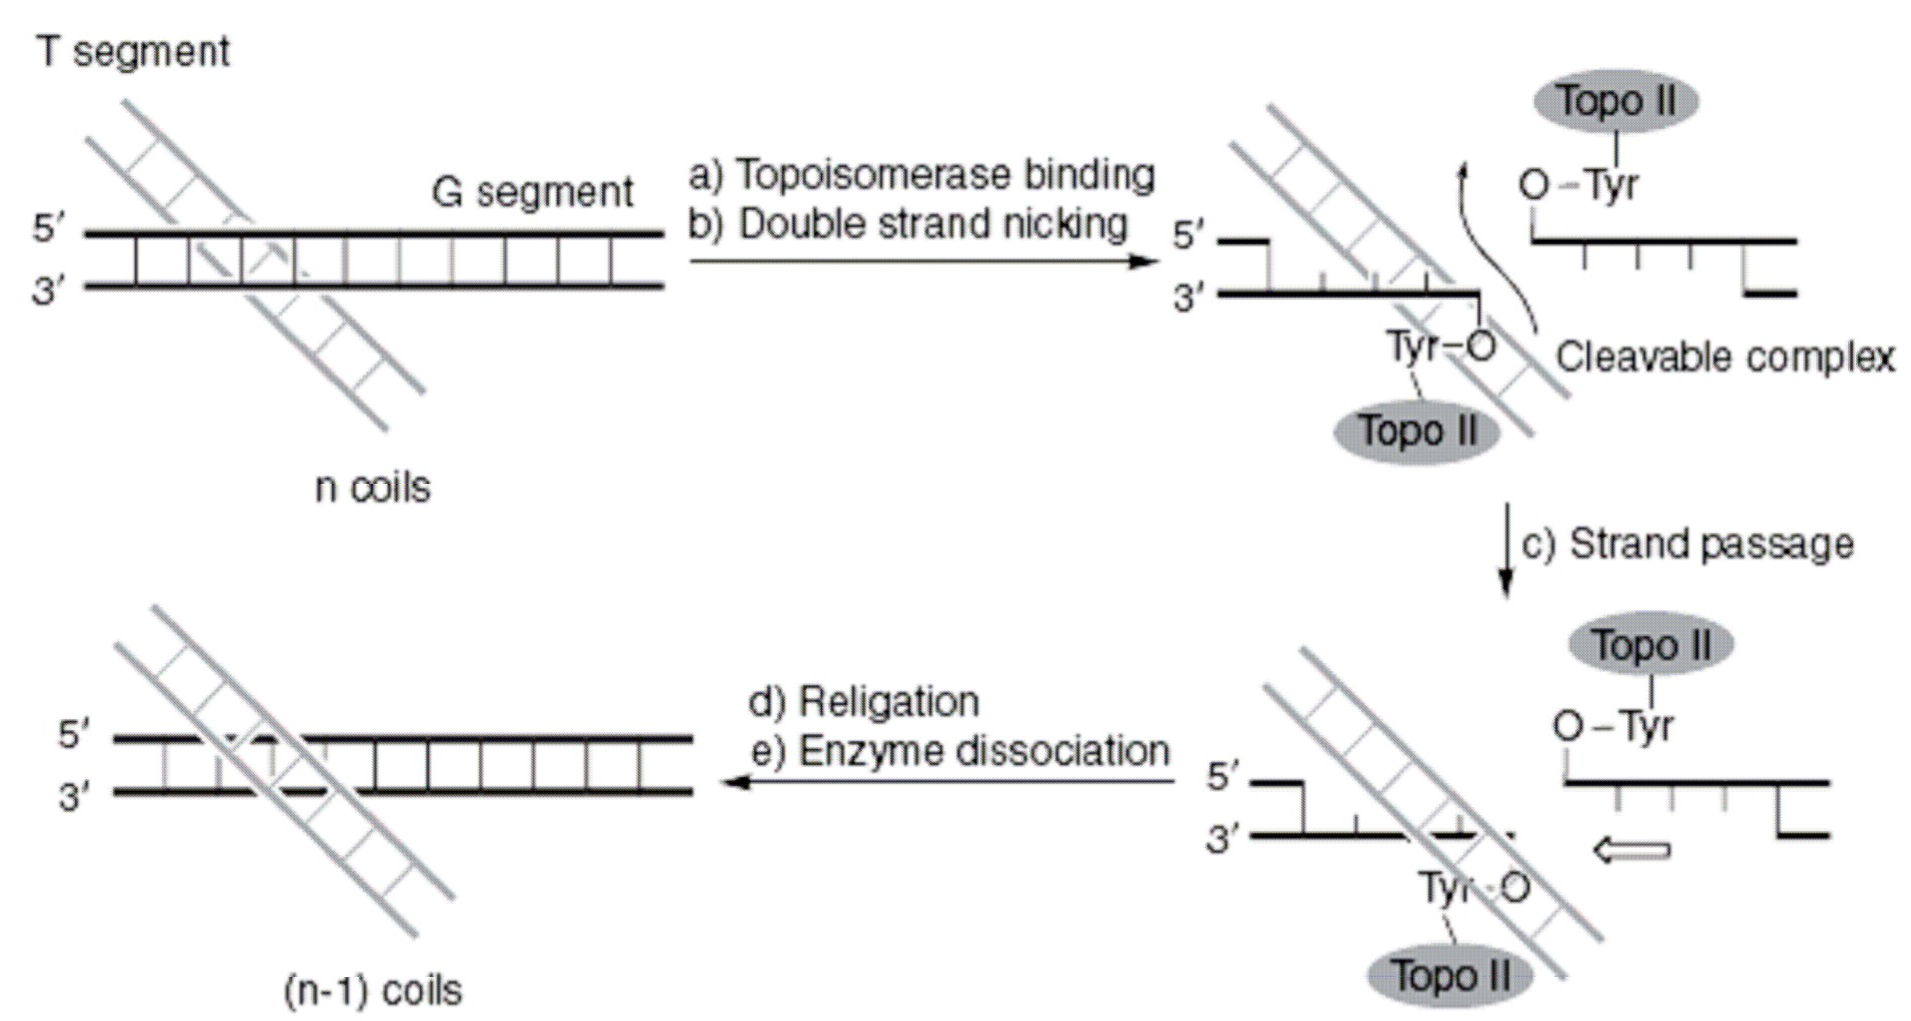
\includegraphics[width=\textwidth]{19_006}
\end{figure}

Si forma il complesso di Cleavable, in seguito si ha il rilassamento
della catena di DNA e in seguito si ha la chiusura. Il processo avviene
tante volte, quanto è necessario per avere una certa topologia del DNA.

Questo meccanismo può essere avvelenato. Quando l'elica è intercalata da
un farmaco, l'enzima non può rilegarsi. Questo causa un danno permanente
al DNA.

Non agendo direttamente sulla proteina, il processo viene definito
\emph{avvelenamento} dell'enzima.

L'avvelenamento comporta che il double strand di DNA non sia rilegato,
quindi si induce il meccanismo di apoptosi, che consente all'organismo
di eliminare la cellula.

La selettività di questo intervento farmacologico, è elevata. In una
cellula in rapida evoluzione è presente in quantità maggiore e con
un'attività elevata, quindi si interferisce maggiormente con cellule che
si riproducono velocemente. Comunque un intercalante va a intaccare
tutte le cellule\ft{Se si lavora con sostanza intercalanti, è necessario portare proteggersi.}.

Questa strategia può essere utilizzata contro i batteri, che posseggono
la topoisomerasi IV

\fullpicture*{19_005}{Topoisomerasi II}
\fullpicture*{19_007}{Avvenenamento dell'enzima}

\clearpage

\section{Antracicline}

Le antracicline sono veleni delle topoisomerasi II. Sono degli agenti intercalanti. Sono
selettive per le cellule in rapida evoluzione.

Le antracicline più utilizzate sono la \emph{Doxorubicina} e la \emph{Daunorubicina}. L'unica
differenza tra le due è il gruppo \ce{OH}, la Doxorubicina è più potente e viene
usata per tumori solidi piuttosto che liquidi, mentre la Daunorubicina è
efficace solo per la leucemia.
Sono sostanze citotossiche; noi usiamo questa tossicità per i nostri
interessi, ovvero eliminare le cellule tumorali

Sono composti da un sistema aromatico planare, che consente lo stacking
con le basi del DNA. Sono anche idrofile e permettono di avere delle
interazioni ad idrogeno.

\marginpicture*{19_008}{Doxorubicina e Daunorubicina}

I gruppi sono evidenziati nell'immagine \ref{fig:Antra}. La parte verde è responsabile
dell'intercalazione in DNA. Le molecole hanno una intercalazione
preferenziale in appaiamento G-C, e si ha una certa disposizione nei
solchi maggiori della porzione a sinistra; mentre lo zucchero protende
verso il solco minore.
La porzione in rosso indica che c'è una ammina protonabile, e che può
esserci del legame ad idrogeno.

\begin{figure}[H]
  \centering
  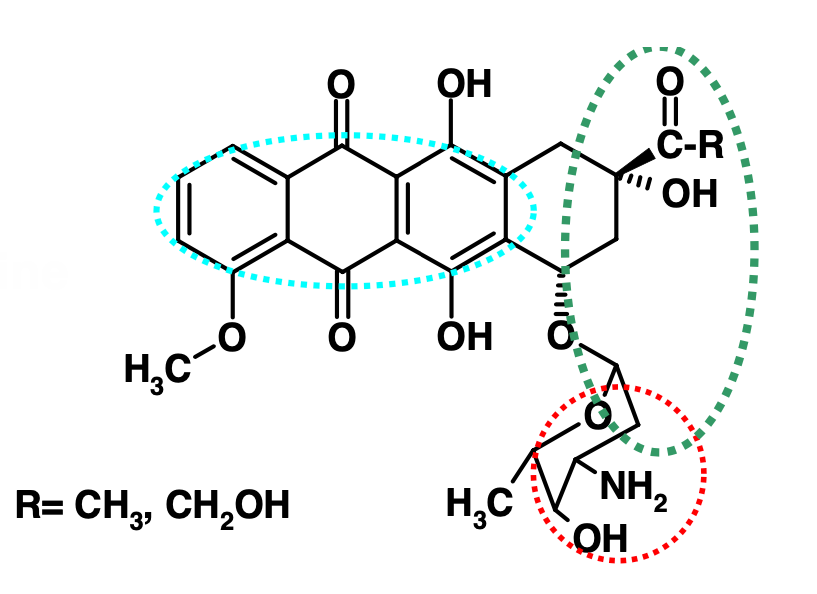
\includegraphics[width=0.45\textwidth]{19_009}
  \caption{Struttura delle antracicline}
  \label{fig:Antra}
\end{figure}

Queste molecole non legano il gruppo fosfato nel solco maggiore o
minore, ma protendono, quindi sono vicine ma non legate, impedendo il
legame della proteina. La possibilità di avere una carica consente di
approcciare la doppia elica che presenta l'esterno carico negativamente.
Queste due molecole vengono somministrate per via iniettiva

\marginpicture*{19_010}{Mitoxantrone}

Dalle antracicline, si è passato alla sintesi di molecole con lo stesso
tipo di interazione, con il \emph{mitoxantrone}. La porzione aromatica è
triciclica, quindi la struttura è stata semplificata. La molecola è
simmetrica è quindi è più facile da sintetizzare.

In questo caso non si ha la porzione dello zucchero, in quanto si
riteneva che gli effetti cardiotossici del farmaco derivano dallo
zucchero, quindi per limitare gli effetti collaterali è stata rimossa.
Il sostituente amminico è stato mantenuto ed è stato inserito
all'interno delle catene laterali. Le catene laterali vengono esposte
verso il solco minore.

Si ha uno schema interattivo ripetuto due volte.

\marginpicture*{19_011}{Amsacrina}

Un altra classe di farmaci è rappresentata dalla \emph{amsacrina}, dove il core
rimane circa uguale. La catena diventa aromatica e viene introdotto un
gruppo elettron-attrattore.

Queste sono le classi di farmaci di avvelenamento delle topoisomerasi
II, e impediscono la ricucitura del filamento.

